\documentclass{math}

\usepackage{tikz}

\title{University Physics 2}
\author{Alvin Lin}
\date{January 2018 - May 2018}

\begin{document}

\maketitle

\section*{Electric Potential}
Conservation of Energy:
\[ \Delta K+\Delta U = W_{ext} \]
The change in potential energy plus the change in kinetic energy is equal to
the external work by non-conservative forces. If there is no outside work:
\begin{align*}
  \Delta K+\Delta U &= 0 \\
  E_i &= E_f \\
  K_i+U_i &= K_f+U_f
\end{align*}
\( K \) is usually \( \frac{1}{2}mv^2 \) while \( U \) depends on the specifics
of the problem. Also recall the formula for work:
\[ W = \vec{F}\cdot\Delta\vec{r} \]
With many different forces:
\[ W = \sum\vec{F}\cdot\Delta\vec{r_i} \]
\( \vec{F} \) will generally not be constant, which requires us to integrate:
\[ W = \int_{i}^{f}\vec{F}\cdot\diff{\vec{r}} \]
If a potential energy is doing the work:
\[ W = -\Delta U_{internal} \]
For electrial fields, we will start with:
\[ W = \int\vec{F}\cdot\diff{r} \]
and plug in forces from electric fields.
\begin{align*}
  W &= \int\vec{F}\cdot\diff{\vec{r}} \\
  &= \int(q\vec{E})\cdot\diff{\vec{r}} \\
  &= qE\Delta x \\
  \Delta U &= -W = -qE\Delta x \\
  \text{Electric potential} &= \Delta V = \frac{\Delta U}{q} = -E\Delta x
\end{align*}
Electric potential is measured in volts, where one volt is equal to one joule
per Coulomb.

\subsection*{Equipotential Lines}
Equipotential lines are like a topographic map. Along an equipotential line,
voltage and potential energy are constant (these are scalars, not vectors,
\( \Delta V = 0 \)). So along a line:
\[ W = -\Delta U = -q\Delta v = 0 \]
No work is done, nor does potential energy change:
\[ W = \int\vec{F}\cdot\diff{\vec{r}} = \int(q\vec{E})\cdot\diff{\vec{r}} = 0 \]
For all fields: \( \vec{E}\bot\diff{\vec{r}} \). The electric field is
perpendicular to the equipotential lines at all points and points from high to
low. The region with the largest electric field is where the equipotential
lines are closest together.

\subsection*{Work/Energy}
\begin{align*}
  W &= -\Delta U = -q\Delta V = \int_{i}^{f}\vec{F}\cdot\diff{r} \\
  \Delta V &= -\frac{1}{q}\int_{i}^{f}\vec{F}\cdot\diff{\vec{r}} \\
  &= -\int_{i}^{f}\frac{\vec{F}}{q}\cdot\diff{\vec{r}} \\
  &= -\int_{i}^{f}\vec{E}\cdot\diff{\vec{r}}
\end{align*}

\subsection*{Voltage Difference for a Point Charge}
If we ask for \( V_r \), this means with respect to infinity, where \( V(\infty)
= 0 \).
\begin{align*}
  \Delta V &= V_{\infty}-V_r = -\int_{r}^{\infty}\vec{E}\cdot\diff{\vec{r}} \\
  V_r &= \int_{r}^{\infty}\vec{E}\cdot\diff{\vec{r}} \\
  \diff{\vec{r}} &= \diff{r'}\hat{r} \\
  V_r &= \int_{r}^{\infty}\frac{kq}{r'^2}\diff{r'} \\
  &= \bigg[-kq\frac{1}{r}\bigg]_{r}^{\infty} \\
  &= \frac{1}{4\pi\epsilon_{\circ}}\frac{q}{r} = \frac{kq}{r}
\end{align*}
With multiple point charges:
\[ V_{total} = \sum_{point~charge} = V_1+V_2+V_3+\dots \]
The potential energy between two point charges is:
\[ \Delta U = q\Delta V = \frac{kq_1q_2}{r} \]
Additionally:
\[ W_{ext} = -W_e = \Delta U \]
To find \( V(r) \) for a charge distribution:
\[ \diff{V} = \frac{k\diff{q}}{r} \]
In summary:
\begin{enumerate}
  \item \( \Delta V = \int\vec{E}\cdot\diff{\vec{r}} \)
  \item \( \Delta V = \int\frac{k\diff{q}}{r} \)
  \item \( \Delta U = q\Delta V \)
\end{enumerate}

\subsubsection*{Example}
These problems are analogous to finding the electric field of a charge
distribution. Assume a constant charge density of \( \lambda \):
\begin{center}
  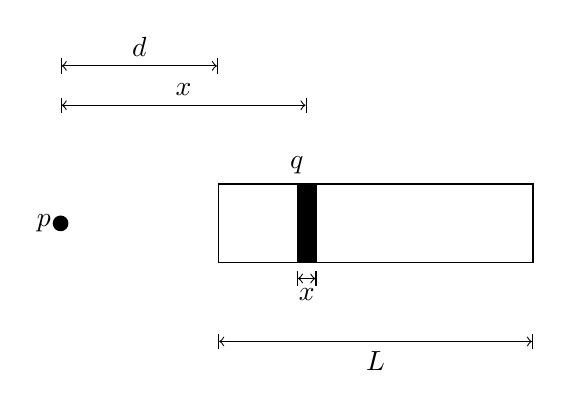
\begin{tikzpicture}
    \draw (0,0) -- (4,0) -- (4,1) -- (0,1) -- cycle;
    \fill (-2,0.5) circle (0.1cm) node[left] {\( p \)};
    \fill (1,0) -- (1.25,0) -- (1.25,1) -- (1,1) node[above] {\( \diff{q} \)};
    \draw[|<->|] (-2,2.5) -- (0,2.5) node[pos=0.5,above] {\( d \)};
    \draw[|<->|] (-2,2) -- (1.125,2) node[pos=0.5,above] {\( x \)};
    \draw[|<->|] (1,-0.2) -- (1.25,-0.2) node[pos=0.5,below] {\( \diff{x} \)};
    \draw[|<->|] (0,-1) -- (4,-1) node[pos=0.5,below] {\( L \)};
  \end{tikzpicture}
\end{center}
\begin{align*}
  \diff{V} &= \frac{k\diff{q}}{x} \\
  &= \frac{k\lambda\diff{x}}{x} \\
  V &= \int_{d}^{d+L}\frac{k\lambda\diff{x}}{x} \\
  &= k\lambda\bigg[\ln(x)\bigg]_{d}^{d+L} \\
  &= k\lambda\ln\bigg(\frac{d}{d+L}\bigg)
\end{align*}
Unlike the electric field problems, the voltage is a scalar, so we don't need
to break it into its components. The voltage is also proportional to
\( \frac{1}{r} \) instead of \( \frac{1}{r^2} \).

\subsection*{Finding the Electric Field from Voltage}
We know the following:
\[ V_b-V_a = -\int_{a}^{b}\vec{E}\cdot\diff{\vec{r}} \]
Also by definition:
\[ V_b-V_a = \int_{a}^{b}\diff{V} \]
Therefore:
\begin{align*}
  \int_{a}^{b}\diff{V} &= -\int_{a}^{b}\vec{E}\cdot\diff{\vec{r}} \\
  \diff{V} &= -\vec{E}\cdot\diff{\vec{r}} \\
  \diff{r} &= \diff{x}\i+\diff{y}\j+\diff{z}\k \\
  -\diff{V} &= E_x\diff{x}\i+E_y\diff{y}\j+E_z\diff{z}\k \\
  E_x &= -\pdiff{V}{x} \quad E_y = -\pdiff{V}{y} \quad E_z -\pdiff{V}{z} \\
  \vec{E} &= E_x\i+E_y\j+E_z\k \\
  &= -\bigg(\pdiff{V}{x}\i+\pdiff{V}{y}\j+\pdiff{V}{z}\k\bigg) \\
  &= -\triangledown V
\end{align*}
Thus the electric field is just the gradient of the voltage.

\begin{center}
  You can find all my notes at \url{http://omgimanerd.tech/notes}. If you have
  any questions, comments, or concerns, please contact me at
  alvin@omgimanerd.tech
\end{center}

\end{document}
